
\chapter{Encoding of Assembly Instructions to Machine Code}
\label{ch-njmcencoding}

{\small
\begin{flushright}
Design: David; Documentation: David, Cristina; Implementation: David [Mar 99]
\end{flushright} 
}

This chapter describes a 1999 investigation into dynamic executions of
software and binary encoding of intermediate representations using the NJMC
toolkit encoding routines.  The objective of this exercise was to take an
assembly input, encode the instructions into machine code and execute the
output instructions at run-time.  This exercise resulted in RAE, a
Run-time Assembler Executor, which is described in this chapter. 

The ultimate goal for this software is to take an RTL-based 
representation and be able to generate machine code that is executed
on the target machine.
The dynamic behaviour of RAE should also be implemented by allowing 
switching between each component on-the-fly.  On-demand processing also 
enforces task switch as data are executed and gathered as needed.
This component can then be plugged into the backend of dynamic
binary translators or emulators.


\section{Design and Implementation}

The current RAE implementation can process SPARC assembly programs and execute
encoded binaries on the SPARC (V8 for both input and output).  x86
implementation shall be followed once the SPARC version of RAE can handle
RTL-based input.  The input assembly files are produced by
VPO~\cite{Beni88} as we are hoping to use VPO as an optimizer in static
binary translations.  Test files used for testing RAE are programs written
in the C language.  To get the assembly version, VPCC is used to compile
the programs in to assembly file.  Note: VPCC understands K\&R syntax
only. 

\centerfigbegin
\resizebox{!}{8cm}
{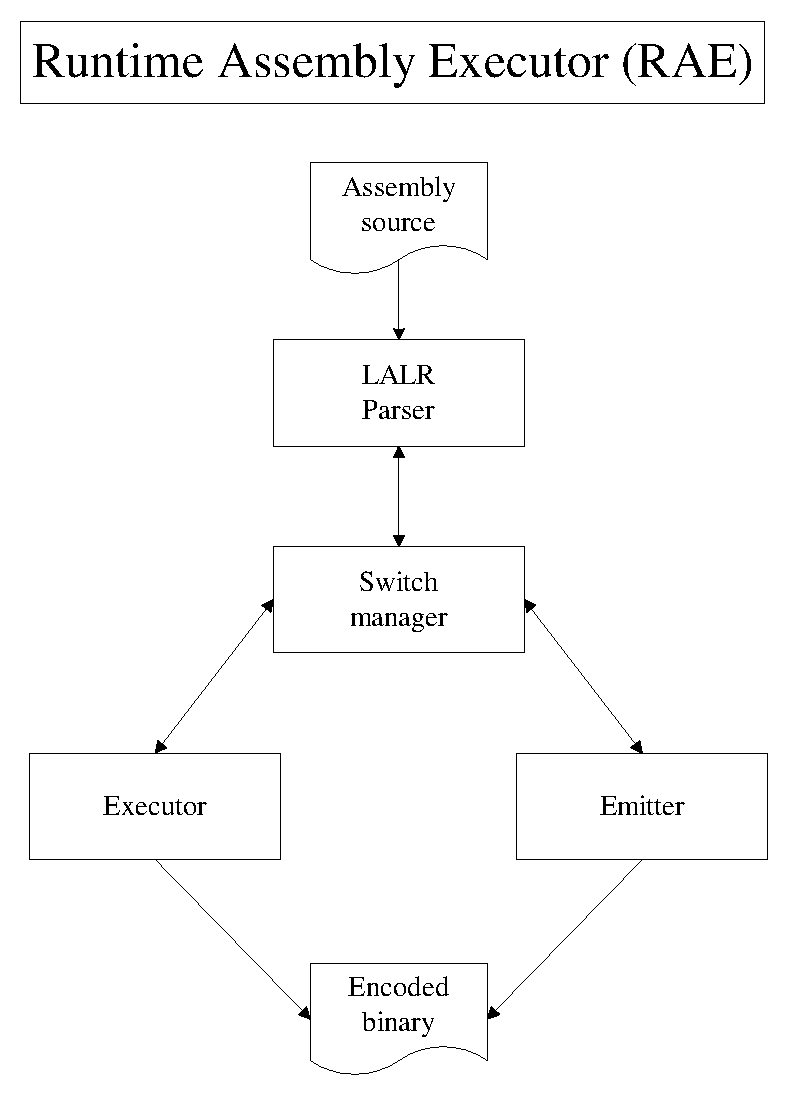
\includegraphics{figures/rae.eps}}
\centerfigend{fig-rae}{Components of RAE}

RAE is made up by 4 main components (see Figure~\ref{fig-rae}):  

\begin{itemize} 
\item 	The parser, 
		which parses VPO-generated assembly files using a LALR parser. 
		Structures, relocations, label information are gathered as each unit 
		of input is parsed.  Details regarding the parser are
		explained in more detail in the following subsections. 

\item 	The emitter, which uses NJMC toolkit encoding routines to encode the
		assembly instructions into binary instructions.  The emitter is invoked
		mainly by the parser and is reponsible for outputing the final binaries
		needed by the executor. 

\item 	The executor, which executes the translated binary code at run-time. 
	
\item 	The switch manager, which maintain the connections between the above
		components.  It jobs is to direct the flow of translation\/program 
		execution and the communications between the components such that 
		on-demand processing can be achieved.  
\end{itemize}

The dynamic behaviour of RAE results mainly from the ability to process
on-demand in the individual components.  Processing of each component are
done only when there is a need to do so.  For example, when the emitter
emits enough information for execution, the executor is invoked.  The
executor is then paused when there is a call to a label which it does not
yet know about, hence it invokes the parser to parse more source in search
for the desire label.  Each component are closely coupled in a way that
they are triggered on-demand.  Granularity of RAE can be seen as
processing one procedure at a time in the parser component. 


\section{RAE Parser} 
The parser is the first to be called by RAE.  
In a sequencial order, the parser starts at the top of the assembly file and
processes the input in an orderly fashion.  
The granularity unit of the parser is a single procedure at a time.  
The parser must gather enough information from the input file such that other
components can be invoked.  
During the parse, the parser invokes the emitter for every instruction that 
needs to be emitted.  
The combination of parsing and emitting pauses once the entry point to the 
main program is found in which the executor is called to execute the encoded
instructions.
Sometime during the running of the program, the switch manager may invoke the 
parser to parse more assembly input as needed.

Each procedure is consider to have a text segment and a local data segment.  
The first procedure
starting from the begining of the file and have no text segment.  It has a
single data segment which stores the labels that are accesible by the rest
of the program.  This is the only procedure that has no code segment and
it is the global data segment.  This segment is responsible to have names
and labels that are used throughout the rest of the program which are not
found in there local data segments.  Apart from being a single segment
procedure, this segment contains data that are similar to the rest of the
procedure's local data segments (at least in the eyes of the parser, they
are treated the same). 


\subsection{Data Segments} 

Data segments are static piece of memory that are allocated before the 
execution of the program.  
These segments may contains both initialised and uninitialised data.
Two types of data segments can be found in an assembly input file: 
texttt{global} and texttt{local} data segments.
The global data segment contains variables and label references that can be
accessed anywhere throughout the program.  
Contents within the local data segment are known only to its corresponding 
text segment.

\subsection *{Input to the parser}

The following assembly constructs are found in data segments within the input
file.

\begin{itemize} 
\item 	\texttt{.seg "data"} - this signifies the beginning of a data segment.
It is at this point that a new data relocatable block is created.  
Relocatable block are base structures provided by the NJMC toolkit. 

\item	\texttt{.align NUM} - NUM is usually 4, 8 or 16.  
a call to the align(NUM) routine is made whenever this is encoutered. 

\item	\texttt{.common VAR,SIZE,ALIGN} - variable VAR is declared with 
size SIZE, and its byte aligned to ALIGN.  
Call to align(ALIGN) is made first, VAR is added to the global symbol 
table if it have not been already added, SIZE bytes
is emited to the current relocatable block using emitm().  Since no
initial value is required, the emitter simply emits junk (currently set to
be the integer 2) for the .common identifier.  For example, in the
following variable declaration \\ \texttt{.common cm\_var, 1024, 4} \\ the
name \texttt{cm\_var} will be added to the symbol table with its offset
from the beggining of the global data segment.  The RAE then emits a
series of 1024 bytes with the value of 2 to specify that the address is
occupied through a series of calls to \texttt{emitm} (which handles
incrementing the \texttt{PC} counter and allocating space if the maximum
buffer space is reached). Another way to do this would be to call
\texttt{addlc()} which simply increments the \texttt{PC} counter. 
Although using \texttt{addlc()} is considerably quicker, extra code needs
to be added to performs similar housekeeping functions in \texttt{emitm}
like checking buffer overfloads if the relocatable block have just been
created.  addlc() can be safely used if a previous call the emitm() has
been made since the creation of the relocatable block.  If addlc() is the
first to be called after a new relocatable block, then some house keeping
is definately required. 

\item	\texttt{.global NAME} - signifies NAME is a global name that can 
be accessed anywhere in the program.  
NAME is added to the global symbol table and a
relocatable address for the NAME label is also created. 

\item	\texttt{LABEL:} - signifies a data label definition.  
If LABEL is not already in
the symols table (searches local symbols first then globals), it will be
added and a relocatable address is created aswell. 


The following belong within a LABEL 

\begin{itemize} 
\item .byte XXXX, 
\item .word XXXX, 
\item .double XXXX,
\item .ascii XXXX - the values XXXX associated with these tags are simply emited
to the current relocatable block. 
\end{itemize}

\end{itemize}

The input assembly file is generated from VPO, but its organisation
of data and text segments make it difficult for a single parse.  
For each text segment, there is always a corresponding local data segment 
(which could be empty).  
The organisation of the VPO assembly will start with the
global data segment, follow by the first text and local data segment pair,
then the second pair etc...  in that order.  Each pair of the text and
local segments is grouped as a single procedure by the parser.  Problem
with a single parse over the input file arises when encountering
references to local data variable its corresponding the text segment. 
Since its local data segment comes after its text segment, no reference
information about variables are known at the point of emiting an
instruction.  To overcome this problem, each local data segment could be
moved infront of its repectable text segment.  This can be very tedious
when the input file contains a large number of procedures.  To fixes this
problem, relocation closures are used.  Relocation closures are created
when an unknown symbol (or address) is referenced in the text segment. 
When the symbol is discovered (in its corresponding local segment), the
closure is applied to the instruction that created the relocation closure. 
This is done by patching the instruction space with the correct relocation
address. 

\subsection *{Example}

The following example code demonstrates the processing done during the
parse: 

input code:  
\begin{verbatim}
.seg "text"             (1)  
.align 8                (2)  
.global .L45            (3)  
.L45:                   (4) 
save %sp, -96, %sp      (5)  
sethi %hi(.L60), %o0    (6)  
add %o0, %lo(.L60), %o0 (7) 
...  
...  
.seg "data"             (8)  
.align 8                (9)  
.L60:                   (10)  
.word 0x46ff            (11)  
... 
\end{verbatim}

At the entry to the procedure, the parser allocates a new relocatable
block and does some housekeeping (1).  At (3), the symbol .L45 is added to
the global symbols table (global so that other procedures can call .L45). 
A label for .L45 is also created but not defined.  (4) defines label .L45
by assigning it the current offset from the beginning of the relocatable
block.  A save instruction is emited to the relocatable block by invoking
the respective emitter function (5).  As it encouters .L60 in (6), it
attempts to lookup the global symbols table in search for .L60 and fails. 
The parser adds .L60 to the local symbols table and creates a label for
it.  It then invokes the emitter which creates a relocation closure for
this instruction.  (7) uses .L60 again, this time the parser finds .L60 in
its local symbols and asks the emitter to emit the add instruction.  But
the emitter detects that .L60 is not defined and created another
relocation closure.  When the text segment is completed, the parser
creates another relocatable block for its local data segment(8).  At (10),
the parser defines .L60.  At (11), 0x46ff is emitted to the relocatable
block. 

As the RAE parser parses the VPO assembly output, it builds 2 (except the
first procedure) relocatable block for each procedure it encounters along
with a symbol table for all the symbols that are define in this procedure. 
When the parser finishes parsing a procedure, it tries to fix all the
incomplement instructions during the parse by applying the closures.  As
each closure is being appled, it patches over incomplete instruction with
the correct target address of the labels. 

Notice that the first procedure does not have a text segment.  This
procedure contains the global data section, hence the symbols table for
this procedure contains all the symbols and labels that are global to the
entire program.  This table defines variables that are accessible during
program execution. 

For succesful instruction encoding using global and local variable address
references and run-time execution, an exact copy of the disk image is
created in memory.  At the end of a procedure parse and after closures are
applied, information within each relocatable block are copied to a
contiguous piece of memory that is suitable for execution. 


\subsection{Text} 
As each procedure is being parsed, each assembly
instruction is determined, mapped and constructed by issuing a call to the
emmiter (see section 1.3) which invokes the corresponding NJMC encoding routine.  For example, for the assembly instruction 

\begin{verbatim}
	add %o0, 10, %o0 
\end{verbatim}

A call to the \texttt{add} function is made by the emitter to emit the
actual instruction to the text relocatable block. 

To process procedure call instructions, the parser looks up the global
symbol table and decides the next set of actions:  \begin{itemize} \item
For labels (infact, symbols as well) that are defined in the symbols
table, an explicit call instruction to the label's address is encoded. 
\item For labels not found in the table, the parser checks if the label
	exists in the libraries used by the program (currently only
	\texttt{libc.so.1} is checked). 
	If so, it is implemented as an indirected call.  Indirected calls
	are patched with two instructions---\texttt{sethi} and
\texttt{jmpl}. 
	The former instruction takes the address of the library routine,
	puts it into register \texttt{\%g5}, then a jump and link
(\texttt{jmpl})
	follows.  \item For unknown label, a call to the switch manager is
made.  The parser creates a new label for the destination of the call. 
Since the address of the destination is unknown at the time of encoding,
the
	name of the procedure that's being called is also passed to the
	switch manager. 
	See the section in On-demand to see how the switch manager is
used. \end{itemize}

The processing of branches is similar to that of calls for labels that
have been defined.  Branch targets that are unknown will result in
generating a relocation closure for the instruction with the target label
added to the local symbols table.  Branch target is never in the
libraries.

Closures are applied at the end of the parsing phase.  All fix ups within
intructions are handled by looping through the set of closures and
applying each in turn.  For address that are still undetermined during
closure analysis, the program will simply fail with an error.


\subsection{Others} In the case of loads and stores during the parsing of
the input file, the parser needs to indentify and encode the appropriate
instructions. Both version of float and integer loads uses the same
\texttt{ld} mnemonic but their opcodes are different.  The parser
determines whether the instruction involves floating point registers and
encodes the instruction accordingly---\texttt{ld} for integer loads and
\texttt{ldf} for floating point loads.


\section{RAE emitter} The RAE's emitter is automatically generated by the
NJMC tookit using the Sparc encoding specifications.  Communication
between the parser and the emitter is through the functions found in
\texttt{sparc.h}.  This file provides encoding functions that will
produces machine binaries for each Sparc instruction. 


\subsection{NJMC toolkit}

The NJMC toolkit can use a machine instruction specification to create
both encoding and decoding routine.  In this report, I will be discussing
encoding only.  The routines that can be used for encoding (as are used in
RAE) are generated by running xtools over the Sparc specification files. 
Function names are generated with relation to the names used in the spec
files.  eg. the add instruction will be implemented with the C function
ADD(rs1, reg\_or\_imm, rs2). 


\section{RAE executor} Control is parsed to the RAE executor with the
entry address of the main program.  The executor executed the encoded
instruction just like any other piece of code in memory.  The name of
executor is gcode, and its assign a value when the address of main is
found.  The executor is invoke by calling gcode() explicitly. 


\section{On-demand} One significant change from RAE rev 1 to rev 2 is the
introduction of on-demand processing.  On-demand processing allows
parsing, emiting and executing of code that are only requied at run-time. 

For each procedure parsed by the RAE parser, 2 relocatable blocks and 1
symbols table is constructed (except the first procedure).  The emitter is
invoked during the parse and actual instructions and data are emited
within the relocatable block.  At the end of a parse (end of one
procedure), all the relocation closures are apply.  Copies of each
relocatable to a contiguous piece of memory is done before the RAE parser
starts parsing another procedure. 

The RAE parser will parse the input file until the main procedure is
found.  Program execution start as soon as main is parsed and emited.  For
all other piece of code that are not yet parsed at this point in time, a
call to the "switch manager" is generated to take its place.  When a
program needs to call a procedure "proc1" yet to be parsed, instead it
calls the switch manager.  The switch manager looks up the list of
procedure that it knows about and tries to find "proc1".  If sucessful,
"proc1" is called.  If "proc1" does not exist in the known procedure list,
the switch manager asks the parser to parse another procedure until
"proc1"  is found and the code is emited.  When "proc1" is found, the
switch manager no only passes control to "proc1", it also patches the
original call to the switch manager with a call to "proc1". 

Example code before and after patching. 

original code to from input

\begin{verbatim}
add %o0, 0x188, %o0 
call proc1, 2 
add %o1, 0x302, %o1
\end{verbatim}

When call to "proc1" needs to be emited, the emitter emits a call to the
switch manager instead (instructions 0x60a70 and 0x60a74).  In order for
the switch manager to know that "proc1" is the required procedure, the
address containing the string "proc1" is also emited (instructions 0x60a68
and 0x60a6c). 

\begin{verbatim}
0x60a64 <_end+32108>:  add %o0, 0x188, %o0 
0x60a68 <_end+32112>:  sethi %hi(0x5bc00), %g5 
0x60a6c <_end+32116>:  add %g5, 0x258, %g5      ! 0x5be58 <_end+12640> 
0x60a70 <_end+32120>:  sethi %hi(0x13c00), %g6 
0x60a74 <_end+32124>:  call %g6 + 0x3b4         ! 0x13fb4 <switch_manager>
0x60a78 <_end+32128>:  add %o1, 0x302, %o1
\end{verbatim}

After the switch manager have found the address for "proc1" (through calls
to the parser and emitter in search for "proc1"), it patches the call to
the switch manager with a straight call to "proc1".  It also removes the
instructions at 0x60a68 and 0x60a6c. 

\begin{verbatim}
0x60a64 <_end+32108>:  add %o0, 0x188, %o0 
0x60a68 <_end+32112>:  nop
0x60a6c <_end+32116>:  nop 
0x60a70 <_end+32120>:  sethi %hi(0x62000), %g5
0x60a74 <_end+32124>:  call %g5 + 0x390 		! 0x62390 <_end+38552> 
0x60a78 <_end+32128>:  add %o1, 0x302, %o1
\end{verbatim}

Because the switch manager is do self modifying code, flush instructions
is needed to flush the cache such that it reflect what is now in memory. 
A jump to the procedure "proc1" is made at the end of the switch manage
